\documentclass[11pt]{article}

\usepackage[a4paper,margin=1in]{geometry}
\usepackage{fontspec}
\usepackage{xeCJK}
\usepackage{xcolor}
\usepackage{hyperref}
\usepackage{booktabs}
\usepackage{longtable}
\usepackage{array}
\usepackage{seqsplit}
\usepackage{enumitem}
\usepackage{listings}
\usepackage[most]{tcolorbox}
\usepackage{titlesec}
\usepackage{fancyhdr}
\usepackage{parskip}
\usepackage{tikz}
\usetikzlibrary{arrows.meta,positioning}

\IfFontExistsTF{PingFang SC}{\setCJKmainfont{PingFang SC}}{\setCJKmainfont{Songti SC}}
\IfFontExistsTF{Helvetica Neue}{\setmainfont{Helvetica Neue}}{\setmainfont{Arial}}
\IfFontExistsTF{Menlo}{\setmonofont{Menlo}}{\setmonofont{Courier New}}

\definecolor{axonblue}{HTML}{1F4E79}
\definecolor{axongray}{HTML}{4A5568}
\definecolor{axonlight}{HTML}{F6F8FA}
\definecolor{axonred}{HTML}{9B1C1C}
\definecolor{axongreen}{HTML}{166534}
\definecolor{axonamber}{HTML}{92400E}

\hypersetup{colorlinks=true,linkcolor=axonblue,urlcolor=axonblue}
\pagestyle{fancy}
\setlength{\headheight}{14pt}
\fancyhf{}
\lhead{EasyNet 状态机器现实审计}
\rhead{2026-06-09}
\cfoot{\thepage}

\titleformat{\section}{\Large\bfseries\color{axonblue}}{\thesection}{0.6em}{}
\titleformat{\subsection}{\large\bfseries\color{axongray}}{\thesubsection}{0.6em}{}

\newcommand{\code}[1]{{\ttfamily\scriptsize\expandafter\seqsplit\expandafter{\detokenize{#1}}}}
\newcommand{\statecode}[1]{{\ttfamily\scriptsize\expandafter\seqsplit\expandafter{\detokenize{#1}}}}
\newcolumntype{L}[1]{>{\raggedright\arraybackslash}p{#1}}

\newtcolorbox{auditbox}{
  colback=axonlight,
  colframe=axonblue,
  title=现实审计规则,
  fonttitle=\bfseries,
  arc=1mm
}

\newtcolorbox{gapbox}{
  colback=white,
  colframe=axonred,
  title=缺口,
  fonttitle=\bfseries,
  arc=1mm
}

\lstdefinestyle{easynet}{
  basicstyle=\ttfamily\small,
  backgroundcolor=\color{axonlight},
  frame=single,
  rulecolor=\color{axongray},
  breaklines=true,
  columns=fullflexible
}
\lstset{style=easynet}
\sloppy
\emergencystretch=4em

\tikzset{
  state/.style={rectangle,rounded corners=1mm,draw=axonblue,fill=axonlight,align=center,minimum width=2.45cm,minimum height=0.72cm,font=\scriptsize},
  fail/.style={rectangle,rounded corners=1mm,draw=axonred,fill=white,align=center,minimum width=2.45cm,minimum height=0.72cm,font=\scriptsize},
  edge/.style={-{Latex[length=1.8mm]},thick,draw=axongray}
}

\title{\textbf{EasyNet 状态机器现实审计与修正版}\\
\large 当前代码事实、RFC-005 目标契约与未收敛缺口}
\author{EasyNet Engineering}
\date{2026-06-09}

\begin{document}
\maketitle

\begin{abstract}
本文修正早期只描述 clean target 的状态机草稿。本文把当前代码已经实现的事实、RFC-005 的目标契约、仍未收敛的缺口分开陈述, 覆盖 \code{join/start}、namespace resolve、invoke、Backend HTTP read model、Frontend typed state、\code{runtime stop} 与 reset/self-uninstall。没有源文件证据的状态不会被写成已实现。
\end{abstract}

\tableofcontents
\newpage

\section{更正结论}

\begin{auditbox}
前一版文档的问题是把目标架构、当前代码和缺口混在一起。本文要求每个状态机同时给出 \code{Current implementation}、\code{Target contract}、\code{Gap}。没有源文件证据的状态只能写成目标, 不能写成当前事实。
\end{auditbox}

核心结论如下:
\begin{itemize}[leftmargin=*]
  \item \code{JoinConnectionState} 已经存在, 但状态码不是一一对应, 不足以定位所有中断状态。
  \item \code{runtime start} 已经在 credential verify、Hub session endpoint、daemon boot failure 上记录 snapshot, 且 join autostart 失败会显式报错。
  \item \code{runtime stop} 当前是命令阶段对象, 不是持久化产品状态机。
  \item \code{reset} 当前是 local unpair/reset, 不是完整 self uninstall/leave。
  \item Backend prepare/submit 已基本切到 resolver-selected route; read-model、media、download、history 仍有迁移缺口。
  \item Axon resolver negative reason 只能使用 proto/RFC-005 固定集合, runtime 文本应进入 failure locator detail。
\end{itemize}

\section{建模规则}

\begin{longtable}{L{0.26\linewidth} L{0.20\linewidth} L{0.18\linewidth} L{0.25\linewidth}}
\toprule
状态机 & Owner & 当前完整度 & 说明 \\
\midrule
Join credential/runtime admission & CLI & 部分完整 & 有 snapshot, code 粒度不足 \\
Runtime start/session/presence & CLI daemon + Hub & 部分完整 & 需要更强 admission evidence \\
Namespace resolve & Axon + CLI daemon & 协议完整, 产品未全收敛 & ResolveAnswer 已规范 \\
Invocation/receipt & Axon + Backend + CLI & 部分完整 & producer failure receipt 未全覆盖 \\
Backend HTTP read model & Backend & 部分完整 & pages 局部迁移, 仍有字符串解析 \\
Frontend connected/degraded & Frontend & 部分完整 & invoke route-aware, media 仍解析字符串 \\
Runtime stop & CLI & 缺产品状态机 & StopPlan 不是持久化状态 \\
Reset/self uninstall & CLI + Backend/Hub & 缺失 & reset 不等于 uninstall \\
\bottomrule
\end{longtable}

\section{当前代码审计}

\begin{itemize}[leftmargin=*]
  \item \textbf{Join snapshot}: \code{EasyNet-Cli/src/runtime/join_connection_state.rs}. 当前已定义 \code{JoinConnectionState}、\code{JoinTransition}、\code{JoinFailureCode}、\code{JoinConnectionSnapshot}; 缺口是多个状态共用同一 code。
  \item \textbf{Join autostart}: \code{EasyNet-Cli/src/facade/cli/join.rs}. pairing accepted 后默认 start daemon; start 失败显式报错。
  \item \textbf{Runtime start}: \code{EasyNet-Cli/src/facade/cli/start.rs}. credential verify、Hub endpoint probe、daemon boot failure 都记录 snapshot; 仍需保证 online 只在 session admission evidence 后记录。
  \item \textbf{Stop}: \code{EasyNet-Cli/src/facade/cli/stop.rs}. 当前有 \code{StopPlan/StopStage}; 缺少持久化 stop state/code。
  \item \textbf{Reset}: \code{EasyNet-Cli/src/facade/cli/reset.rs}. active runtime 时拒绝 reset; best-effort revoke 后删除本地 credentials; 当前不是 self uninstall。
  \item \textbf{Backend route facade}: \code{EasyNet/backend/internal/logic/ability/resolve_invoke_route.go}. 已经调用 daemon resolver; negative 转 typed validation error。
  \item \textbf{Backend prepare/submit}: \code{prepareEnvelopeLogic.go}, \code{submitSignedInvocationLogic.go}. prepare 使用 selected route; submit 校验 prepare-time route binding。
  \item \textbf{Backend pages}: \code{listPagesLogic.go}, \code{helpers.go}. pages unavailable DTO 局部存在; 仍通过错误字符串判断 offline/not advertised。
  \item \textbf{Frontend invoke DTO}: \code{Frontend/src/lib/api/easynet-abilities.ts}. \code{target_ura/tool_name} 已存在, failure locator 类型存在。
  \item \textbf{Frontend media}: \code{Frontend/src/store/media-channel-*.ts}. 仍匹配 PresenceRegistry 字符串, 需要 typed failure。
  \item \textbf{macOS client}: \code{EasyNet-Client/.../DeviceConnectionManager.swift}. 仍可能合成 \code{ability_ura}; 应删除 canonical URA synthesis。
  \item \textbf{Axon namespace proto}: \code{EasyNet-Axon/core/proto/axon/v1/namespace.proto}. ResolveAnswerKind 和 NegativeReason 已规范。
  \item \textbf{Axon receipt proto}: \code{EasyNet-Axon/core/proto/axon/v1/invoke.proto}. \code{InvocationReceipt.failure} 已存在; producer 覆盖不足。
\end{itemize}

\section{Join / Runtime Start 状态机}

\subsection{当前实现状态}

\begin{longtable}{L{0.25\linewidth} L{0.08\linewidth} L{0.23\linewidth} L{0.30\linewidth}}
\toprule
Current state & Code & Wire state & 问题 \\
\midrule
\code{PairingNone} & J000 & \code{PAIRING_NONE} & OK \\
\code{PairingTokenPending} & J100 & \code{AUTH_TOKEN_READY} & 与 preflight/consumed 混码 \\
\code{PairingTokenPreflighted} & J100 & \code{AUTH_TOKEN_READY} & 与 pending 混码 \\
\code{PairingTokenExpired} & F510 & \code{JOIN_REJECTED} & OK \\
\code{PairingTokenConsumed} & J100 & \code{JOIN_REQUESTED} & 不应与 pending 混码 \\
\code{DeviceValidatedJoining} & J200 & \code{PAIRING_ACCEPTED} & OK \\
\code{CredentialsSaved} & J300 & \code{HUB_PREFLIGHT} & 与 trust/preflight 混码 \\
\code{LocalTrustWired} & J300 & \code{HUB_PREFLIGHT} & 与 credential 混码 \\
\code{RuntimeStarting} & J400 & \code{DAEMON_BOOT} & 与 daemon booting 混码 \\
\code{HubCredentialVerified} & J300 & \code{HUB_PREFLIGHT} & 与本地保存混码 \\
\code{HubSessionEndpointReachable} & J300 & \code{HUB_PREFLIGHT} & 与 credential 混码 \\
\code{DaemonBooting} & J400 & \code{DAEMON_BOOT} & 与 runtime starting 混码 \\
\code{SelfSessionAdmissionPending} & J500 & \code{SESSION_CONNECTING} & OK \\
\code{ConnectedOnline} & J800 & \code{FRONTEND_CONNECTED} & 与 suspect/draining 混码 \\
\code{ConnectedSuspect} & J800 & \code{DEGRADED} & 不应与 online 混码 \\
\code{ConnectedDraining} & J800 & \code{OFFLINE} & 不应与 online 混码 \\
\code{DisconnectedRemoved} & F530 & \code{OFFLINE} & 与 unknown 混码 \\
\code{ConnectionUnknown} & F530 & \code{OFFLINE} & 与 removed 混码 \\
\code{Failed} & F000 & \code{FAILED} & 应减少使用 \\
\bottomrule
\end{longtable}

\subsection{目标状态码}

\begin{longtable}{L{0.10\linewidth} L{0.34\linewidth} L{0.28\linewidth} L{0.18\linewidth}}
\toprule
Code & Target state & Transition in & Surface \\
\midrule
J000 & \code{PAIRING_NONE} & none & doctor \\
J100 & \code{PAIRING_TOKEN_PENDING} & \code{T01_CREATE_PAIRING} & frontend \\
J110 & \code{PAIRING_TOKEN_PREFLIGHTED} & \code{T02_PREFLIGHT_TOKEN} & CLI \\
F120 & \code{PAIRING_TOKEN_EXPIRED} & token validation & CLI/frontend \\
F130 & \code{PAIRING_TOKEN_CONSUMED} & token validation & CLI/frontend \\
J200 & \code{DEVICE_VALIDATED_JOINING} & \code{T03_VALIDATE_TOKEN} & CLI \\
J300 & \code{CREDENTIALS_SAVED} & \code{T04_SAVE_CREDENTIALS} & doctor \\
J310 & \code{LOCAL_TRUST_WIRED} & \code{T05_WIRE_LOCAL_TRUST} & doctor \\
S300 & \code{RUNTIME_STARTING} & \code{T08_BOOT_DAEMON} & runtime status \\
S310 & \code{HUB_CREDENTIAL_VERIFIED} & \code{T06_VERIFY_CREDENTIAL} & doctor \\
S320 & \code{HUB_SESSION_ENDPOINT_REACHABLE} & \code{T07_CONNECT_SESSION_ENDPOINT} & doctor \\
S330 & \code{DAEMON_BOOTING} & \code{T08_BOOT_DAEMON} & runtime status \\
S340 & \code{SELF_SESSION_ADMISSION_PENDING} & \code{T09_OPEN_SELF_SESSION} & daemon status \\
N500 & \code{NAMESPACE_VISIBLE} & \code{T10_ADMIT_PRESENCE} & backend \\
C700 & \code{CONNECTED_ONLINE} & \code{T11_REFETCH_READ_MODEL} & frontend \\
C710 & \code{CONNECTED_SUSPECT} & degraded event & frontend \\
C720 & \code{CONNECTED_DRAINING} & \code{T12_REMOVE_PRESENCE} & frontend \\
C790 & \code{DISCONNECTED_REMOVED} & presence removed & frontend \\
C791 & \code{CONNECTION_UNKNOWN} & missing evidence & frontend \\
\bottomrule
\end{longtable}

\subsection{状态图}

\begin{center}
\resizebox{\linewidth}{!}{
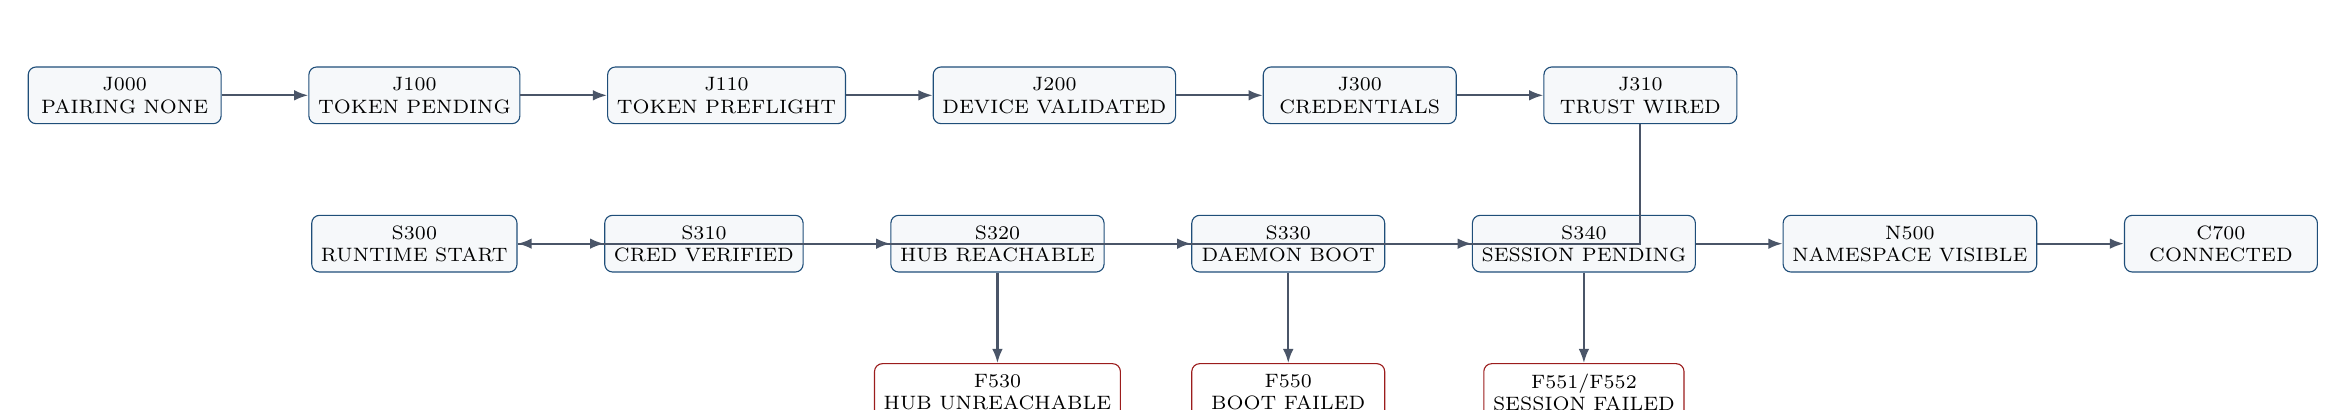
\begin{tikzpicture}[node distance=1.15cm and 1.1cm]
\node[state] (j000) {J000\\PAIRING NONE};
\node[state,right=of j000] (j100) {J100\\TOKEN PENDING};
\node[state,right=of j100] (j110) {J110\\TOKEN PREFLIGHT};
\node[state,right=of j110] (j200) {J200\\DEVICE VALIDATED};
\node[state,right=of j200] (j300) {J300\\CREDENTIALS};
\node[state,right=of j300] (j310) {J310\\TRUST WIRED};
\node[state,below=of j100] (s300) {S300\\RUNTIME START};
\node[state,right=of s300] (s310) {S310\\CRED VERIFIED};
\node[state,right=of s310] (s320) {S320\\HUB REACHABLE};
\node[state,right=of s320] (s330) {S330\\DAEMON BOOT};
\node[state,right=of s330] (s340) {S340\\SESSION PENDING};
\node[state,right=of s340] (n500) {N500\\NAMESPACE VISIBLE};
\node[state,right=of n500] (c700) {C700\\CONNECTED};
\node[fail,below=of s320] (f530) {F530\\HUB UNREACHABLE};
\node[fail,below=of s330] (f550) {F550\\BOOT FAILED};
\node[fail,below=of s340] (f551) {F551/F552\\SESSION FAILED};
\draw[edge] (j000) -- (j100);
\draw[edge] (j100) -- (j110);
\draw[edge] (j110) -- (j200);
\draw[edge] (j200) -- (j300);
\draw[edge] (j300) -- (j310);
\draw[edge] (j310) |- (s300);
\draw[edge] (s300) -- (s310);
\draw[edge] (s310) -- (s320);
\draw[edge] (s320) -- (s330);
\draw[edge] (s330) -- (s340);
\draw[edge] (s340) -- (n500);
\draw[edge] (n500) -- (c700);
\draw[edge] (s320) -- (f530);
\draw[edge] (s330) -- (f550);
\draw[edge] (s340) -- (f551);
\end{tikzpicture}
}
\end{center}

\subsection{Failure 修正}

\begin{longtable}{L{0.12\linewidth} L{0.30\linewidth} L{0.32\linewidth} L{0.14\linewidth}}
\toprule
Code & Failure & Interrupted transition & Retryable \\
\midrule
F500 & \code{JOIN_FAILED_PREFLIGHT} & \code{T02_PREFLIGHT_TOKEN} & maybe \\
F510 & \code{JOIN_FAILED_VALIDATE} & \code{T03_VALIDATE_TOKEN} & no/maybe \\
F520 & \code{START_FAILED_CREDENTIAL_VERIFY} & \code{T06_VERIFY_CREDENTIAL} & maybe \\
F530 & \code{HUB_UNREACHABLE} & \code{T07_CONNECT_SESSION_ENDPOINT} & yes \\
F550 & \code{DAEMON_BOOT_FAILED} & \code{T08_BOOT_DAEMON} & yes/maybe \\
F551 & \code{SELF_SESSION_ADMISSION_FAILED} & \code{T09/T10} & maybe \\
F552 & \code{SESSION_RUNTIME_UNAVAILABLE} & \code{T09_OPEN_SELF_SESSION} & yes \\
F560 & \code{RESOLVE_UNAVAILABLE} & \code{T11_REFETCH_READ_MODEL} & yes \\
\bottomrule
\end{longtable}

\begin{gapbox}
用户看到的 \texttt{dendrite bridge library not found} 不应再粗略归入 \code{DAEMON_BOOT_FAILED}; 目标应投影成 \code{F552} \code{SESSION_RUNTIME_UNAVAILABLE}, interrupted transition 为 \code{T09_OPEN_SELF_SESSION}。
\end{gapbox}

\section{Namespace Resolve 状态机}

Axon 的合法 answer kind 是 \code{NON_DISPATCHABLE}、\code{DELEGATION}、\code{FINAL_ROUTE}、\code{NEGATIVE}。合法 negative reason 是 \code{UNSPECIFIED}、\code{NXDOMAIN}、\code{NODATA}、\code{NOROUTE}、\code{STALE}、\code{UNAUTHORIZED}、\code{THROTTLED}、\code{OVERLOADED}、\code{REFUSED}、\code{LOOP}。

\begin{longtable}{L{0.22\linewidth} L{0.18\linewidth} L{0.44\linewidth}}
\toprule
Resolve state & Dispatch allowed & Required output \\
\midrule
\code{FINAL_ROUTE} & yes & selected \code{ability_ura}, \code{route_ura}, \code{dispatch_name}, \code{next_hop}, evidence \\
\code{DELEGATION} & no local dispatch & peer hub or delegated authority \\
\code{NEGATIVE} & no & negative reason, canonical failure code, locator \\
\code{NON_DISPATCHABLE} & no & catalog/resource metadata only \\
\code{RESOLVE_UNAVAILABLE} & no & source, stage, retryable, message \\
\bottomrule
\end{longtable}

\section{Invoke 状态机}

通用路径是:

\begin{lstlisting}
User action or CLI command
  -> ResolveQuery
  -> ResolveAnswer.FinalRoute
  -> prepare canonical envelope
  -> client signs
  -> submit
  -> admission
  -> dispatch resolver-selected next_hop
  -> exactly one terminal InvocationReceipt
\end{lstlisting}

\begin{longtable}{L{0.24\linewidth} L{0.34\linewidth} L{0.30\linewidth}}
\toprule
Variant & Expected next hop & Extra failure cases \\
\midrule
同用户同 realm 同设备 & \code{LocalDeviceAbility} 或 daemon local & ability absent, local execution failed \\
同用户同 realm 其他设备 & hub/device session route & PresenceRegistry miss, stale route \\
同用户跨 realm & delegation then peer final route & realm not found, delegation refused \\
跨用户同 realm & policy-authorized hosted/device route & policy denied/hidden, owner not found \\
跨用户跨 realm & peer delegation + peer policy & delegation refused, unauthorized \\
Hosted agent ability & \code{HostedAgentViaDevice} & agent not advertised, host device offline \\
Hub/local ability & \code{LocalHubAbility} & hub overloaded, ability not found \\
Streaming/download & final route + stream contract & body committed before failure, trailer needed \\
Terminal/resource producer & final route + receipt & producer must fill \code{InvocationReceipt.failure} \\
\bottomrule
\end{longtable}

\subsection{Canonical failure code}

RFC-005 主分类必须使用: \code{REALM_NOT_FOUND}, \code{REALM_DELEGATION_REFUSED}, \code{ALIAS_LOOP}, \code{ALIAS_AUTHORITY_INVALID}, \code{TARGET_NOT_FOUND}, \code{OWNER_NOT_FOUND}, \code{ABILITY_NOT_FOUND}, \code{ABILITY_OWNER_SHADOWED}, \code{ABILITY_QUERY_CONFLICT}, \code{ROUTE_NOT_FOUND}, \code{ROUTE_STALE}, \code{RESOURCE_NOT_FOUND}, \code{RESOURCE_SCOPE_DENIED}, \code{POLICY_DENIED}, \code{POLICY_HIDDEN}, \code{CAPACITY_THROTTLED}, \code{EXECUTION_OVERLOADED}, \code{NO_DISPATCHABLE_NEXT_HOP}, \code{RESOLVER_PROFILE_NOT_AUTHORITATIVE}, \code{EXECUTION_FAILED}。

\section{Backend HTTP 与 Frontend 状态}

\begin{longtable}{L{0.30\linewidth} L{0.28\linewidth} L{0.30\linewidth}}
\toprule
Situation & Correct HTTP shape & Product meaning \\
\midrule
DB rows exist, resolver unavailable & 200 + rows + \code{resolve_unavailable[]} & stale/degraded read model \\
route negative & typed 400/422 & action invalid now \\
daemon/bridge unavailable & typed 503 & retryable runtime unavailable \\
auth/policy denied & typed 403 & permission problem \\
backend invariant violation & typed 500 & backend bug \\
\bottomrule
\end{longtable}

Frontend 只能从 Backend typed DTO、resolver catalog route、receipt failure、download trailer/control frame 渲染状态。不能从空列表或 human string 推断 connected/offline。

\section{Runtime Stop 状态机}

当前 \code{stop.rs} 已有较好的命令对象分层: \code{StopShape}, \code{StopPlan}, \code{StopStage}。缺口是它没有持久化状态码, 所以 doctor 无法回答“stop 停在哪个 transition”。

\begin{longtable}{L{0.12\linewidth} L{0.36\linewidth} L{0.30\linewidth}}
\toprule
Code & Target state & Current stage \\
\midrule
O000 & \code{STOP_REQUESTED} & command start \\
O100 & \code{STOP_SHAPE_CLASSIFIED} & \code{StopPlan::from_state} \\
O200 & \code{REVOKE_PRESENCE} & \code{stage_revoke} \\
O300 & \code{STOP_HEARTBEAT} & \code{stage_stop_heartbeat} \\
O400 & \code{STOP_DAEMON} & \code{stage_stop_daemon} \\
O500 & \code{SWEEP_DAEMONS} & \code{stage_sweep_daemons} \\
O600 & \code{STOP_AXON_RUNTIME} & \code{stage_stop_axon_runtime} \\
O700 & \code{CLEANUP_RUNTIME_STATE} & \code{stage_cleanup_state} \\
O900 & \code{STOPPED} & success \\
\bottomrule
\end{longtable}

\section{Reset 与 Self Uninstall}

当前 \code{reset.rs} 是 local reset/unpair。完整 self uninstall/leave 应拆成独立语义:

\begin{longtable}{L{0.28\linewidth} L{0.40\linewidth} L{0.20\linewidth}}
\toprule
Command & Meaning & Failure policy \\
\midrule
\texttt{easynet reset} & local credential/runtime cleanup & 可继续, 但必须记录 partial \\
\texttt{easynet self uninstall/leave} & authoritative Hub-side leave + local cleanup & remote failure 必须 terminal 或 explicit partial \\
\bottomrule
\end{longtable}

目标 self uninstall 状态:
\begin{lstlisting}
U000 UNINSTALL_REQUESTED
  -> U100 RUNTIME_GUARD
  -> U200 REVOKE_SESSION
  -> U300 REMOVE_HUB_MEMBERSHIP
  -> U400 REMOVE_LOCAL_TRUST
  -> U500 DELETE_CREDENTIALS
  -> U600 CLEANUP_RUNTIME_FILES
  -> U900 UNINSTALLED
\end{lstlisting}

\section{RFC-005 计划对齐审计}

本节修正一个关键问题: 状态机器不能只写 clean target。必须和 Axon 仓库已经固定的 RFC-005 计划包以及当前代码对齐。规范来源包括 \code{005-ura-namespace-resolution-dns-plan.md} 以及 \code{00-intent.md} 到 \code{06-decisions-log.md}。结论是: Axon 中 authoritative resolver 状态机器已经存在, 产品仓库必须向它收敛; CLI/Backend/Client 不能再自建 route inference。

\subsection{Axon 当前代码事实}

\begin{longtable}{L{0.18\linewidth} L{0.44\linewidth} L{0.26\linewidth}}
\toprule
Gate & Code evidence & Result \\
\midrule
A1 typed owner parser & \code{EasyNet-Cli/src/ura.rs} re-export \code{easynet_axon::ura::*}; \code{AbilitySelector} 只做投影。 & CLI 方向正确。 \\
A2 proto & \code{core/proto/axon/v1/namespace.proto} 定义 \code{NegativeReason}, \code{ResolveAnswerKind}, \code{NextHop}, \code{ResolveAnswer}. & Axon proto 已有。 \\
A4 resolver object & \code{core/runtime-rs/src/services/namespace/resolver.rs} 定义 \code{NamespaceRouteResolver} 和 \code{V1Resolver}. & Axon runtime 已有对象边界。 \\
A6 invoke consume & \code{core/runtime-rs/src/services/invocation/resolver_consume.rs} 消费 \code{ResolveAnswer}; \code{rpc_handlers.rs} 分支处理 FinalRoute/Delegation/Negative/NonDispatchable. & 带 \code{easynet.target_ura} 的 invoke 已接入。 \\
A7 release profile & \code{profile.rs} 从 Preview 起步; \code{resolver_consume.rs} 对非 product-dispatchable profile 机械拒绝 dispatch/forward。 & 已实现 fail-closed gate。 \\
Receipt failure & \code{invoke.proto} 有 \code{InvocationReceipt.failure = 30}; resolver negative 可映射到带 namespace evidence 的 \code{pb::Error}. & 协议载体已有; producer 覆盖仍需审计。 \\
\bottomrule
\end{longtable}

因此 product invoke 必须包含这个 pre-dispatch gate:
\begin{lstlisting}
I120 RESOLVE_ROUTE
  -> I130 CHECK_RESOLVER_PROFILE
      Preview/ShadowRead + FinalRoute/Delegation
        -> I902 NO_DISPATCHABLE_NEXT_HOP
      AuthoritativeLocal/Production + FinalRoute
        -> I300 LOCAL_DISPATCH
      AuthoritativeLocal/Production + Delegation
        -> I400 PEER_DELEGATION
      Negative
        -> I900 TERMINAL_FAILURE
      NonDispatchable
        -> I902 NO_DISPATCHABLE_NEXT_HOP
\end{lstlisting}

\subsection{当前跨仓库未收敛点}

\begin{longtable}{L{0.18\linewidth} L{0.40\linewidth} L{0.30\linewidth}}
\toprule
Repo & Observed code & RFC-005 risk \\
\midrule
EasyNet-Cli & \code{src/eal/interpreter.rs} 仍用 \code{TargetOwnedAbilityUra::from_selector} 后调用 federation forward。 & EAL child invoke 可能绕过 resolver-selected route。 \\
EasyNet-Cli & \code{src/runtime/agents/invoke_ability.rs} input schema 仍要求 \code{ability_ura}. & 只能作为 internal/diagnostic; 产品路径不能要求 naked ability URA。 \\
EasyNet-Cli & \code{src/runtime/failure_codes.rs} 仍按 PresenceRegistry/not advertised 文本分类。 & failure projection 仍不是完全 canonical。 \\
Backend & \code{backend/internal/runtime/pty_driver.go} 构造 \code{axon.PublishedAbilityURA(calleeURA, ability)}. & PTY 路径仍在 Backend 侧合成 device-owned ability URA。 \\
Backend & \code{backend/internal/logic/page/helpers.go} 用字符串判断 pages host offline。 & pages failure 还未完全 typed negative。 \\
Backend & \code{backend/internal/handler/file/pumps.go} 已写 \code{X-EasyNet-Failure} trailer。 & 后端侧部分完成; browser/client 解码仍需核验。 \\
Frontend & \code{media-channel-invocation.ts} 和 \code{media-channel-store.ts} 仍匹配 \code{not in PresenceRegistry}. & UI 仍消费 transport 文本而不是 FailureLocator。 \\
EasyNet-Client & macOS 旧函数名 \code{Ability.synthesizeAbilityURI} 生成 \code{/agents/.../abilities/...@version}. & 与 RFC-005 最终 URA grammar 不兼容。 \\
\bottomrule
\end{longtable}

\subsection{修正后的 invoke 状态族}

不能再用一个泛化 invoke 图隐藏 route class。正确模型是公共前缀加显式分支:
\begin{lstlisting}
COMMON
  I000 REQUEST_RECEIVED
  I020 VALIDATE_TARGET_URA_AND_TOOL_NAME
  I040 LOAD_CALLER_SUBJECT_AUTHORITY
  I080 BUILD_RESOLVE_QUERY
  I120 RESOLVE_ROUTE
  I130 CHECK_RESOLVER_PROFILE

SAME REALM FINAL ROUTE
  I300 DISPATCH_LOCAL_OR_REMOTE_SELECTED_ROUTE
  I500 EMIT_TERMINAL_RECEIPT
  I900 COMPLETED

CROSS REALM DELEGATION
  I400 FORWARD_TO_PEER_HUB
  I420 PEER_RESOLVE_AUTHORITATIVELY
  I440 PEER_FINAL_ROUTE_OR_NEGATIVE
  I500 RETURN_RECEIPT_CHAIN
  I900 COMPLETED

NEGATIVE / NON-DISPATCHABLE
  I700 MAP_NEGATIVE_TO_FAILURE_CODE
  I720 ATTACH_FAILURE_LOCATOR
  I740 WRITE_INVOCATION_RECEIPT_FAILURE
  I950 FAILED_TYPED
\end{lstlisting}

\begin{longtable}{L{0.38\linewidth} L{0.28\linewidth} L{0.22\linewidth}}
\toprule
Condition & Receipt code & Locator layer \\
\midrule
unknown realm & \code{REALM_NOT_FOUND} & Realm \\
delegation refused & \code{REALM_DELEGATION_REFUSED} & Authority \\
target absent & \code{TARGET_NOT_FOUND} & Identity \\
owner absent & \code{OWNER_NOT_FOUND} & Owner \\
ability absent with owner present & \code{ABILITY_NOT_FOUND} & Ability \\
full ability URA plus secondary ability name & \code{ABILITY_QUERY_CONFLICT} & Ability \\
no route & \code{ROUTE_NOT_FOUND} & Route \\
stale route lease & \code{ROUTE_STALE} & Route \\
positive but not dispatchable & \code{NO_DISPATCHABLE_NEXT_HOP} & Route \\
resource absent & \code{RESOURCE_NOT_FOUND} & Resource \\
resource scope denied & \code{RESOURCE_SCOPE_DENIED} & Resource/Policy \\
policy denied or hidden & \code{POLICY_DENIED} / \code{POLICY_HIDDEN} & Policy \\
resolve capacity exhausted & \code{THROTTLED} & Route \\
execution plane saturated & \code{OVERLOADED} & Execution \\
\bottomrule
\end{longtable}

\subsection{Join/Stop/Uninstall 修正}

Join 必须把 credential accepted 和 runtime connected 拆开:
\begin{lstlisting}
J000 TOKEN_RECEIVED
J050 PAIRING_PREFLIGHT
J100 PAIRING_ACCEPTED
J150 CREDENTIALS_PERSISTED
J200 BOOT_REQUESTED
J230 BRIDGE_LIB_VALIDATED_OR_NOT_REQUIRED
J260 HUB_SESSION_ENDPOINT_REACHABLE
J300 DAEMON_PROCESS_STARTED
J360 AXON_RUNTIME_READY
J420 SELF_SESSION_ADMITTED
J500 PRESENCE_ADVERTISED
J700 BACKEND_READ_MODEL_VISIBLE
J900 CONNECTED
\end{lstlisting}

Stop 至少持久化:
\begin{lstlisting}
S000 STOP_REQUESTED
S100 SIGNAL_DAEMON
S200 DRAIN_SESSIONS
S300 UNPUBLISH_PRESENCE
S400 STOP_RUNTIME
S500 VERIFY_SOCKET_CLOSED
S900 STOPPED
S950 PARTIAL_STOP
\end{lstlisting}

Self uninstall/leave 至少持久化:
\begin{lstlisting}
U000 UNINSTALL_REQUESTED
U100 RUNTIME_GUARD
U200 REVOKE_SESSION
U300 REMOVE_HUB_MEMBERSHIP
U400 UNPUBLISH_DEVICE_AND_ABILITIES
U500 REMOVE_LOCAL_TRUST
U600 DELETE_CREDENTIALS
U700 CLEAN_RUNTIME_FILES
U900 UNINSTALLED
U950 PARTIAL_UNINSTALL
\end{lstlisting}

\section{修复计划}

\subsection{EasyNet-Cli}
\begin{itemize}[leftmargin=*]
  \item 将 \code{JoinConnectionState::code()} 改成一一对应。
  \item 拆分 boot failure、self-session admission failure、session runtime unavailable。
  \item 确保 \code{ConnectedOnline} 只在 self-session admission/PresenceRegistry evidence 后记录。
  \item 为 stop/reset 增加持久化 lifecycle snapshot。
  \item 所有 ability/resource/meta 调用走 resolver-selected route。
  \item terminal/download/resource producer 统一写 \code{InvocationReceipt.failure}。
\end{itemize}

\subsection{EasyNet Backend}
\begin{itemize}[leftmargin=*]
  \item 保持 \code{resolveSelectedInvokeRouteFrom} 为 prepare route authority。
  \item 审计所有直接要求 \code{ability_ura} 的 handler, 改为 catalog route 或 \code{target_ura + tool_name}。
  \item 删除 page/media/read-model 字符串错误解析, 改 typed failure projection。
  \item read model 返回 degraded DTO; action 返回 typed 4xx/503。
\end{itemize}

\subsection{EasyNet Frontend / Client}
\begin{itemize}[leftmargin=*]
  \item 删除 canonical ability URA synthesis。
  \item 所有 action button 绑定 resolver catalog route。
  \item 用 typed failure locator 替代 PresenceRegistry 字符串匹配。
  \item download client 解码 \code{X-EasyNet-Failure} trailer/control frame。
\end{itemize}

\subsection{EasyNet-Axon}
\begin{itemize}[leftmargin=*]
  \item 保持 NegativeReason 与 RFC-005/proto 一致。
  \item 暴露 runtime/admission/transport error 到 canonical failure code + locator 的 mapper。
  \item 所有 non-success terminal receipt 必须填 \code{InvocationReceipt.failure}。
\end{itemize}

\section{验收标准}

\begin{itemize}[leftmargin=*]
  \item \texttt{easynet join --boot yes} 在 daemon 无法 reach/admit runtime 时失败, 且 snapshot 标出 interrupted transition。
  \item \texttt{easynet doctor --json} 显示 machine、state code、transition、failure locator、next action。
  \item \code{runtime stop} 和 reset/self-uninstall 有稳定状态码。
  \item \code{/api/v1/pages} 不因 agent-not-advertised 返回普通 500。
  \item \code{/api/v1/invocations/history/list} 不再因 route-aware UI 请求报 \code{ability_ura is required}。
  \item \code{meta.list_resources} 有 canonical route 或 typed failure。
  \item Frontend/Client 不再构造 canonical ability URA。
  \item browser/download 能读 typed failure trailer。
  \item failed/timeout/cancelled invocation 都有 \code{InvocationReceipt.failure}。
\end{itemize}

\end{document}
